\documentclass[10pt]{article}

%Math
\usepackage{amsmath}
\usepackage{amsfonts}
\usepackage{amssymb}
\usepackage{amsthm}
\usepackage{ulem}
\usepackage{stmaryrd} %f\UTF{00FC}r Blitz!

%Definitionen / Sätze
\usepackage{thmbox}
\newtheorem[M]{definition}{Def.}
\newtheorem[M]{satz}{Satz}
\numberwithin{equation}{section}


%PageStyle
\usepackage[ngerman]{babel} % deutsche Silbentrennung
\usepackage[utf8]{inputenc} 
\usepackage{fancyhdr, graphicx}
\usepackage[scaled=0.92]{helvet}
\usepackage{enumitem}
\usepackage{parskip}
\usepackage[a4paper,top=2cm]{geometry}
\setlength{\textwidth}{17cm}
\setlength{\oddsidemargin}{-0.5cm}



%My Commands
\newcommand{\RN}{\mathbb{R}} %Real Number
\newcommand{\NN}{\mathbb{N}} %Natural Number
\newcommand{\QN}{\mathbb{Q}} %Rational Number
\newcommand{\ZN}{\mathbb{Z}} %ganze Zahlen
\newcommand{\CN}{\mathbb{C}}
\newcommand{\PN}{\mathbb{P}}
\newcommand{\EN}{\mathbb{E}}
\newcommand{\Bold}[1]{\textbf{#1}} %Boldface
\newcommand{\Kursiv}[1]{\textit{#1}} %Italic
\newcommand{\T}[1]{\text{#1}} %Textmode
\newcommand{\Nicht}[1]{\T{\sout{$ #1 $}}} %Streicht Shit durch

%Arrows
\newcommand{\lra}{\leftrightarrow} 
\newcommand{\ra}{\rightarrow}
\newcommand{\la}{\leftarrow}
\newcommand{\lral}{\longleftrightarrow}
\newcommand{\ral}{\longrightarrow}
\newcommand{\lal}{\longleftarrow}
\newcommand{\Lra}{\Leftrightarrow}
\newcommand{\Ra}{\Rightarrow}
\newcommand{\La}{\Leftarrow}
\newcommand{\Lral}{\Longleftrightarrow}
\newcommand{\Ral}{\Longrightarrow}
\newcommand{\Lal}{\Longleftarrow}

% Code listenings
\usepackage{color}
\usepackage{xcolor}
\usepackage{listings}
\usepackage{caption}
\DeclareCaptionFont{white}{\color{white}}
\DeclareCaptionFormat{listing}{\colorbox{gray}{\parbox{\textwidth}{#1#2#3}}}
\captionsetup[lstlisting]{format=listing,labelfont=white,textfont=white}
\lstdefinestyle{JavaStyle}{
 language=Java,
 basicstyle=\footnotesize\ttfamily, % Standardschrift
 numbers=left,               % Ort der Zeilennummern
 numberstyle=\tiny,          % Stil der Zeilennummern
 stepnumber=5,              % Abstand zwischen den Zeilennummern
 numbersep=5pt,              % Abstand der Nummern zum Text
 tabsize=2,                  % Groesse von Tabs
 extendedchars=true,         %
 breaklines=true,            % Zeilen werden Umgebrochen
 frame=b,         
 %commentstyle=\itshape\color{LightLime}, Was isch das? O_o
 %keywordstyle=\bfseries\color{DarkPurple}, und das O_o
 basicstyle=\footnotesize\ttfamily,
 stringstyle=\color[RGB]{42,0,255}\ttfamily, % Farbe der String
 keywordstyle=\color[RGB]{127,0,85}\ttfamily, % Farbe der Keywords
 commentstyle=\color[RGB]{63,127,95}\ttfamily, % Farbe des Kommentars
 showspaces=false,           % Leerzeichen anzeigen ?
 showtabs=false,             % Tabs anzeigen ?
 xleftmargin=17pt,
 framexleftmargin=17pt,
 framexrightmargin=5pt,
 framexbottommargin=4pt,
 showstringspaces=false      % Leerzeichen in Strings anzeigen ?        
}

%Config
\renewcommand{\headrulewidth}{0pt}
\setlength{\headheight}{15.2pt}

%Metadata
\fancyfoot[C]{If you use this documentation for a exam, you should offer a beer to the authors!}
\title{
	\vspace{5cm}
	Wahrscheinlichkeiten und Statistik
}
\author{Jan Fässler}
\date{5. Semester (HS 2013)}


% hier beginnt das Dokument
\begin{document}

% Titelbild
\maketitle
\thispagestyle{fancy}
\newpage

% Inhaltsverzeichnis
\pagenumbering{Roman}
\tableofcontents	  	


\newpage
\setcounter{page}{1}
\pagenumbering{arabic}

% Inhalt Start

\section{Lapdance \& Kombinatorik}

\subsection{Zufallsexperimente \& Wahrscheinlichkeiten}

\begin{definition}[Zufallsexperiment]
Ein Experiment, welches beliebig oft wiederholt werden kann und bei jeder Durchführung ein Ergebnis aus einer bestimmten Menge von möglichen Ergebnissen annimmt.
\end{definition}

\begin{definition}[Ergebnismenge $\Omega$]
Ein Experiment, welches beliebig oft wiederholt werden Mögliche Ergebnisse eines Zufallsexperiments.
\end{definition}

\begin{definition}[Ergebnis]
Aussage, die bei der Durchführung des Experimentes entweder wahr oder falsch ist, je nachdem welches Ergebnis eingetreten ist.
\end{definition}

\begin{definition}[Wahrscheinlichkeit]
Mass für die relative Häufigkeit mit der das Ereignis bei wiederholten Durchführung des Experimentes eintritt.
\end{definition}

Jedes Ereignis kann als Teilmenge von Ergebnissen interpretiert werden. \\
\\
Die einzelnen Ergebnisse selber können ebenfalls als Ereignisse betrachtet werden: \\
Zu einem Ergebnis $\omega \in \Omega$ gehört das sogenannte \textbf{Elementarereignis} $E = \{\Omega\}$.


\subsection{Laplace-Experiment}
\begin{definition}[Laplace-Experiment]
Ein Zufallsexperiment mit $n$ verschiedenen möglichen Ergebnissen, die alle dieselbe Wahrscheinlichkeit, alse $\frac{1}{n}$ haben.
\end{definition}

Die Wahrscheinlichkeit eines Ereignisses $E \subseteq\Omega$ wird für diesen Fall folgendermassen definiert:
\begin{equation}
  P(E)=\frac{|E|}{|\Omega|}=\frac{\text{Anzahl günstige Ergebnisse}}{\text{Anzahl aller Ergebnisse}}
\end{equation}
Dieses mathematische Modell für ein Laplace-Experiment, bestehend aus der Menge $\Omega$ mit der Funktion $P$ nennt man einen \textbf{Laplace-Raum}. Dieses $P$ heisst auch \textbf{Gleichverteilung}.

\subsection{Kombinatorik}

\subsubsection{Produkte}
\begin{definition}[Produktregel]
Wenn es bei einem mehrstufigen Auswahlprozess für das 1. Objekt $n_1$ Möglichkeiten, für das 2. Objekt $n_2$ Möglichkeiten, \dots , und für das $k$-te Objekt $n_k$ Möglichkeiten gibt, dann gibt es für den gesamten Auswahlprozess $n_1*n_2* \dots * n_k$ Möglichkeiten.
\end{definition}
\begin{center}
	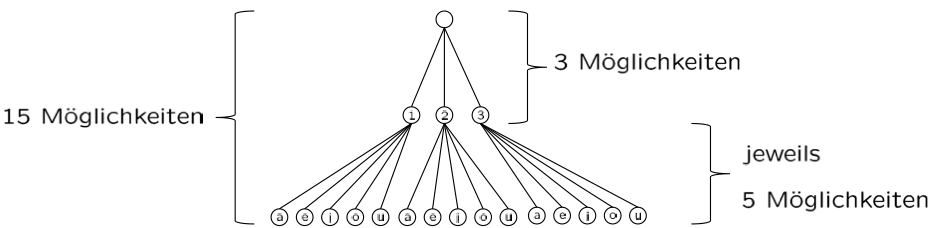
\includegraphics[scale=0.4]{produktregel.png}
\end{center}

\subsubsection{Summen}
\begin{definition}[Summenregel]
Wenn es $n_1$ Objekte mit Eigenschaft 1, $n_2$ Objekte mit Eigenschaft 2, \dots, $n_k$ Objekte mit Eigenschaft $k$ gibt, und kein Objekt zwei der Eigenschaften gleichzeitig besitzt, dann gibt es insgesamt $n_1+n_2+$ \dots $+n_k$ Objekte die eine der Eigenschaft besitzen.
\end{definition}
Beispiel: Eine Meitwagenfirma hat 5 Kleinwagen, 3 Mittelklassewagen und 2 Oberklassewagen. Da kein Auto in mehreren Kategorien sein kann, hat die Firma insgesamt $5+3+2=10$ Wagen.

\subsubsection{Fakultät}
Wir ziehen $n$ mal ohne Zurücklegen mit Beachtung der Reihenfolge aus einer Urne mit $n$ Kugeln. Dan gibt es $n*(n-1)*$ \dots $*2*1$ Möglichkeiten.
\begin{definition}[Fakultät]
Es sei $n \in \NN$. Dann Heisst $n!=n*(n-1)*$ \dots $*2*1$ Fakultät von $n$. Zudem ist $0! := 1$. 
\end{definition}

Es gilt $n! \sim \sqrt{2*\pi*n}*(\frac{n}{e})^n$

\subsubsection{Binominalkoeffizient}
Wir ziehen $k$ mal aus einer Menge von $n$ Zahlen ohne Zurücklegen und ohne Beachtung der Reihenfolge. Es gibt also $\frac{n!}{(n-k)!*k!}$ Möglichkeiten.
\begin{definition}[Binominalkoeffizient]
Es sei $0 \leq k \leq n$. \\
Dann ist der Binominalkoeffizient $\binom{n}{k}$ definiert als $\frac{n!}{(n-k)!*k!}$. \\
Für $k > n$ ist $\binom{n}{k} := 0$.
\end{definition}
$\binom{n}{k}$ gibt also die Anzahl aller $k$-elementigen Teilmengen einer $n$-elementigen Menge an.

\subsection{Urnenmodel}
Viele Abzählprobleme lassen sich auf das sogenannte Urnenmodell zurückführen. Gegeben ist eine Urne mit $n$ unterschiedlichen Kugeln. Wir ziehen $k$ Kugeln aus den $n$ Kugeln. Auf wieviele Arten geht diesm wenn unterschieden wird nach "`Zurücklegen"' oder "`nicht zurücklegen"' und "`geordnet"' oder "`keine Reihenfolge"'? \\
\\
\begin{description}
	\item[k:] Anzahl Ziehungen
	\item[n:] Anzahl Elemente
\end{description}
\begin{tabular}{l|l|l}
 &zur\"{u}cklegen&nicht zur\"{u}cklegen\\\hline
 geordnet&$n^k$&$n!$ oder $\frac{n!}{(n-k)!}$\\\hline
 ungeordnet&$\binom{k+n-1}{k}$&$\binom{n}{k}=\frac{n!}{k!(n-k)!}$
\end{tabular}\\

\newpage
\section{Allgemeine Wahrscheinlichkeiten}
\subsection{Einleitung}
\begin{definition}[Wahrscheinlichkeit]
Eien Wahrscheinlichkeit $P: 2^{\Omega} \rightarrow [0,1]$ erfüllt:
\begin{description}
	\item[(1)] $P(\Omega) = 1$
	\item[(2)] Für endlich oder abzählbar viele parweise disjunktive Ereignisse $E_1,E_2,E_3, $\dots gilt: \\
	 $P(E_1 \cup E_2 \cup E_3 \cup$ \dots $) = P(E_1) + P(E_2) + P(E_3) + $ \dots 
\end{description}
\end{definition}
\begin{satz}
Es sei $P$ eine Wahrscheinlichkeit auf $\Omega$. Dan gilt:
\begin{description}
	\item[(1)] $\forall E \subseteq \Omega : P(E^c)=1-O(E)$
	\item[(2)] $P(0) = 0$
	\item[(3)] $\forall E_1, E_2 \subseteq \Omega : P(E_1\cup E_2) = P(E_1) + P(E_2) - P(E_1 \cap E_2)$
	\item[(4)] Für eine endliche oder abzählbare Menge $E=\{e_1,e_2,$ \dots $\}$ gilt $P(E) = P(\{e_1\}) + P(\{e_2\}) +$ \dots
\end{description}
\end{satz}
Die Wahrscheinlichkeitsverteilung $P$ durch die Angabe der Wahrscheinlichkeiten ist für die Elementarereignisse festgelegt, falls $\Omega$ endlich oder abzählbar ist.
\begin{definition}[Zähldichte (Z-Dichte)]
Die Funktion $f_P : \Omega \rightarrow [0,1]$ mit $f_P(w)=P(\{w\})$ heisst Zähldichte von P.
 \end{definition}
 In diesem Fall gilt also $P(E)=\sum_{e \in E} f_P(e)$, insbesondere $P(E)=\sum_{e \in \Omega} f_P(e)=1$
 
\subsection{bedingte Wahrscheinlichkeit}
Würfeln mit einem normalen Würfel: $\Omega = \{1,2,3,4,5,6\}$, $P=$ Gleichverteilung. Wie hoch ist die Wahrscheinlichkeit  für $A=\{2,3\}$, wenn ich weiss, dass eine ungerade Zahl gewürfelt worden ist? \\
Es verbleibt noch die eingeschränkte Ergebnismenge $B=\{1,3,5\}$. \\
Es sind also nur noch $|B|=3$ Ergebnisse möglich. \\
Davon sind $|A \cap B|=1$ Ergebnisse günstig. \\
Die gesuchte Wahrscheinlichkeit ist somit $\frac{|A \cap B|}{|B|} = \frac{1}{3}$.
\begin{definition}[bedingte Wahrscheinlichkeit]
Es sei $\Omega$ eine nichtleere endliche Menge und $P$ eine Wahrscheinlichkeitsverteilung auf $\Omega$. Ferner sei $B \subseteq \Omega$ mit $P(B) > 0$. \\
Dann heisst $P(A|B) := \frac{P(A \cap B)}{P(B)}$ (elementare) bedingte Wahrscheibnlichkeit von A unter B.
\end{definition} 
\begin{definition}[Formel von Bayes]
Es sei $\Omega$ eine nichtleere endliche Menge und $P$ eine Wahrscheinlichkeitsverteilung auf $\Omega$. Ferner seien $A,B \subseteq \Omega$ mit $P(A) > 0$ und $P(B) > 0$. \\
Dann gilt $P(A|B)=\frac{P(A)}{P(B)} * P(B | A)$.
\end{definition} 
\begin{definition}[totele Wahrscheinlichkeit]
Es sei $\Omega$ eine nichtleere endliche Menge und $P$ eine Wahrscheinlichkeitsverteilung auf $\Omega$. Ferner seien $B_i(i \in I)$ eine Zerlegung von $\Omega$ (d.h. die $B_i$ sind paarweise disjunkt und $\Omega=U_{i \in I} B_i$) mit $P(B_i) > 0$. \\
Dann gilt $P(A) = \sum_{i \in I} P(A | B_i) * P(B_i)$
\end{definition} 
\begin{definition}[positive prädiktive Wert]
Für $0 < P(A) < 1$ gilt mit $\Omega = A \cup A^c$ insbesondere: \\
$P(A | B) = \frac{P(A)*P(A | B)}{P(B | A) * P(A) + P(B | A^c) * P(A^c)}$
\end{definition} 

\subsection{stochastische Unabhängigkeit}
\begin{definition}[stochastisch unabhängig]
Es sei $P$ eine Wahrscheinlichkeitsverteilung auf $\Omega$. \\
Zwei Ereignisse $A,B \subseteq \Omega$ heissen stochastisch unabhängig, falls $P(A \cap B) = P(A) * P(B)$. \\
Im Falle $P(B) \neq 0$ ist dies äquivalent zu $\underbrace{P(A|B)}_{\frac{P(A \cap B)}{P(B)}}=P(A)$.
\end{definition} 

\subsection{Mehrstufige Zufallsexperimente}
Ein $n$-stufiger Versuch mit Ergebnismenge $\Omega_i$ für den $i$-ten Versuch wird meist wie folgt modelliert:
\begin{description}
	\item[(1)] Man legt die Dichte $f_1(\omega_1)$ auf $\Omega_1$ für den ersten Versuch fest.
	\item[(2)] Man legt die Dichte $f_2(\omega_2 | \omega_1)$ auf $\Omega_2$ für den zweiten Versuch in Abhängigkeit vom Ergebnis $\omega_1$ des ersten Versuchs fest.
	\item[(3)] Man legt die Dichte $f_3(\omega_3 | \omega_1, \omega_1)$ auf $\Omega_3$ für den dritten Versuch in Abhängigkeit der Ergebnisse ($\omega_1, \omega_2$) der ersten beiden Versuche fest.
	\item \dots
	\item[(n)] Man legt die Dichte $f_n( \omega_n | \omega_1,$, \dots,$\omega_{n-1}$) auf $\Omega_n$ für den $n$-ten Versuch in Abhängigkeit der Ergebnisse ($\omega_1$, \dots, $\omega_{n-1}$) der ersten $n$ Versuche fest. 
	\item[(n+1)] Die resultierende Dichte auf $\Omega_1$ x $\Omega_2$ x \dots x $\Omega_n$ ist dann $f(\omega_1$, \dots, $\omega_n) = f_1(\omega_1) * f_2(\omega_2 | \omega_1) * $ \dots $ * f_n(\omega_n | \omega_1$, \dots, $\omega_{n-1}$).
\end{description}
Wenn die Versuche nicht voneinander abhängen, dann modelliert man die Versuche einzeln, mit Dichten $f_i(\omega_i)$ auf $\Omega_i$, und erhält als resultierende Dichte $f(\omega_1,$ \dots, $\omega_n)=f1(\omega_1) *$ \dots $* f_n(\omega_n)$. \\
\begin{center}
	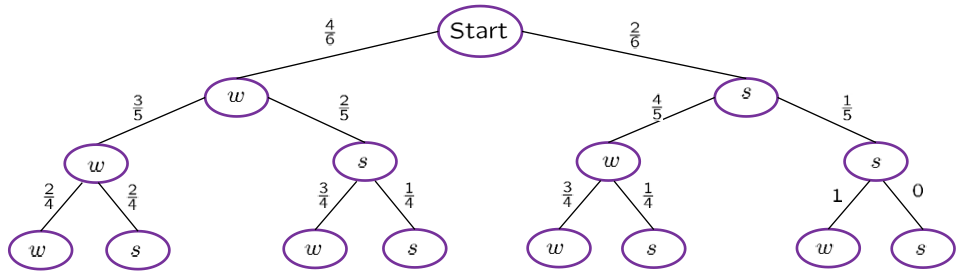
\includegraphics[scale=0.4]{mehrstuffigeW.png}
\end{center}

\newpage
\section{diskrete Zufallsvariablen}
\subsection{Zufallsvariablen}
Eine Zufallsvariable ist eine normale mathematische Funktion. Da bei jeder Durchführung des Zufallsexperiments ein zufälliges Ergebnis $\omega$ eintritt, ist auch der zugehörige Wert $X(\omega)$ nicht vorhersagbar.
\begin{definition}[Zufallsvariable]
Eine Zufallsvariable $X$ über $\Omega$ ist eine Abbildung ovn $\Omega$ in einere Menge $X$. Im Folgenden wird stehts $X \subseteq \RN$ sein. Dan sagt man auch reellwertige Zufallsvariable.
\end{definition}
$X$ induziert eine Wahrscheinlichkeitsverteilung $P^X$ auf $X$ durch $P^X(A)=P(X^{-1}(A))$, wobei $X^{-1}(A)$ das Urbild von A bezeichnet. \\
$P^X$ heisst Verteilung von X oder bildmass von X unter P.

\subsection{Verteilungsfunktion}
\begin{definition}[Verteilungsfunktion]
Es sei $X : \Omega \rightarrow X$ eine Zufallsvariable, wobei $X \in \RN$ eine endliche oder abzählbare Menge ist. Zudem sei $f$ die Zähldichte von $X$. \\
Dann heisst $F(x)=P(X \leq x) = \sum_{t \in X:t \leq x} f(t)$ Verteilungsfunktion von X.
\end{definition}
\begin{center}
	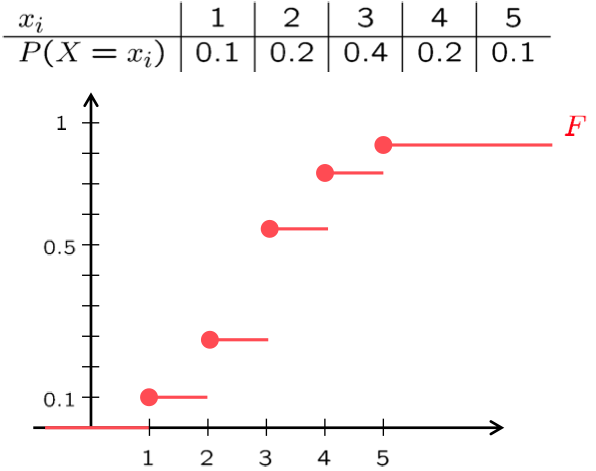
\includegraphics[scale=0.3]{verteilungsfunktion.png}
\end{center}

\subsection{Erwartungswert}
\begin{definition}[Erwartungswert]
Es sei $X : \Omega \rightarrow X$ eine Zufallsvariable, wobei $X \subset \RN$ eine endliche oder abzählbare Menge ist. Zudem sei $f$ die Zähldichte von $X$. \\
Dann heisst $E(X)=\sum_{x \in X} x * f(x)=\sum_{x \in X} x * P(X = x)$ Erwartungswert von X.
\end{definition}

\subsection{Varianz und Standardabweichung}
\begin{definition}[Varianz]
Es sei $X : \Omega \rightarrow X$ eine Zufallsvariable, wobei $X \subset \RN$ eine endliche oder abzählbare Menge ist. Zudem sei $f$ die Zähldichte von $X$ und $\mu$ der Erwartungswert von $X$. \\
Dann heisst $V(X) = \sum_{x \in X} (x - \mu)^2 * f(x) = \sum_{x \in X} (x - \mu)^2 * P(X=x)$ Varianz von $X$.
\end{definition}
Durch das Quadrieren heben sich Abweichung nach unten und nach oben nicht auf, zudem werden grössere Abweichungen stärker gewichtet. \\
\begin{definition}[Standardabweichung]
$\sigma(X) = \sqrt{V(X)}$ heisst Standardabweichung von $X$.\\
\end{definition}
Die Varianz und die Standardabweichung sind MAsse für die Streuung der Zufallsvariable um den Erwartungswert. \\
Zur Berechnung der Varianz ist es manchmal einfacher, folgende Formel zu verwenden:
\begin{satz}
Es sei $X : \Omega \rightarrow X$ eine Zufallsvariable, wobei $X \subset \RN$ eine endliche oder abzählbare Menge ist. \\
Dan gilt $V(X) = E(X^2)-E(X)^2$.
\end{satz}

\subsection{diskrete Verteilung}
\begin{tabular}{l l}
	Alle Ereignisse gleich wahrscheinlich & Laplace \\
	\\
	Treffer$(WK$ $p)$, nicht Treffer & $B(p)$ \\
	\\
	Anzahl Treffer $(WK$ $p)$ in $n$ unabhängigen Versuchen & $Bin(n,p)$ \\
	\\
	Versuche bis erster Treffer $(WK$ $p)$ in unabhängigen Versuchen & $Geo(p)$ \\
	\\
	Verteilung für seltene Ereignisse mit im Schnitt $\lambda$ Ereignissen pro Zeit/Ort-Einheit & $Poi(\lambda)$ \\
\end{tabular}

\subsubsection{Bernoulli-Verteilung}
Treffer$(WK$ $p)$, nicht Treffer
\begin{definition}[Bernoulli-Verteilung]
Die Verteilung einer Zufallsvariable X, die nur zwei Werte 0 (Treffer) oder 1 (kein Treffer) annehmen kann, wobei $p$ die Wahrscheinlichkeit für 1 bezeichent, heisst Bernoulli-verteilt mit Parameter $p$. \\
\end{definition}
Schreibweise: $X \sim B(p)$ \\
Dichte von $X : f(0) = 1 - p$, $f(1) = p$ \\
\\
$E(X) = p$ \\
$V(X) = p*(1-p)$ \\

\subsubsection{Binomial-Verteilung}
Anzahl Treffer $(WK$ $p)$ in $n$ unabhängigen Versuchen
\begin{definition}[Binomial-Verteilung]
Die Verteilung einer Zufallsvariable X, die die Anzahl an Treffern bei der $n$-maligen unabhängigen Durchführung eines Experiments mit zwei Ausgängen, Treffer oder kein Treffer, wobei $p$ die Wahrscheinlichkeit für Treffer bezeichnet, heisst Binomial-verteilt mit Parametern $n,p$. \\
\end{definition}
Schreibweise: $X \sim Bin(n,p)$ \\
Dichte von $X : f(k) = \binom{n}{k} * p^k * (1-p)^{n-k}$, $k=0,1,$ \dots, $n$ \\
\\
$E(X) = n*p$ \\
$V(X) = n*p*(1-p)$ \\
\\
\textbf{Matlab}: binocdf($k$, $n$, $p$)

\subsubsection{geometirsche-Verteilung}
Versuche bis erster Treffer $(WK$ $p)$ in unabhängigen Versuchen 
\begin{definition}[geometischre-Verteilung]
Die Verteilung einer Zufallsvariable X, die die Anzahl der Versuche bis zum ersten Treffer bei der $n$-maligen unabhängigen Durchführung eines Experiments mit zwei Ausgängen, Treffer und kein Treffer, wobei $p$ die Wahrscheinlichkeit für Treffer bezeichnet, heisst geometrisch verteilt mit Parameter $p$. \\
\end{definition}
Schreibweise: $X \sim Geo(n,p)$ \\
Dichte von $X : f(k) = (1-p)^{k-1}*p$, $k=0,1,$ \dots, $n$ \\
$X=k$ bedeutet, dass die ersten $k-1$ Versuche jeweils kein Treffer waren. und der $k$-te Versuch ein Treffer war.
\\
$E(X) = \frac{1}{p}$ \\
$V(X) = \frac{1-p}{p^2}$ \\

\subsubsection{Poisson-Verteilung}
Verteilung für seltene Ereignisse mit im Schnitt $\lambda$ Ereignissen pro Zeit/Ort-Einheit
\begin{definition}[Poisson-Verteilung]
Die Poisson-Verteilung kommt bei Zufallsvariablen zum Einsatz, welche die Anzahl Ereignisse einer bestimmten Art in einer Zeit- und/oder Ort-Intervall beschreiben. Falls im Mittel $\lambda$-Ereignisse auftreten, dann ist X Poisson verteilt mit Parameter $\lambda$. \\
\end{definition}
Schreibweise: $X \sim Poi(\lambda)$ \\
Dichte von $X : f(k) =\frac{\lambda^k}{k!}*e^{-\lambda}$, $k=0,1,$ \dots, $n$ \\
$X=k$ bedeutet, dass die ersten $k-1$ Versuche jeweils kein Treffer waren. und der $k$-te Versuch ein Treffer war.
\\
$E(X) = \lambda$ \\
$V(X) = \lambda$ \\

\subsubsection{Eigenschaften}
\begin{satz}
Es seien $X,Y$ Zufallsvariablen und $a,c \in \RN$.
Dan gilt:
\begin{itemize}
	\item $E(X + Y) = E(X) + E(Y)$ 
	\item $E(a * X) = a * E(X)$
	\item $E(X + c) = E(X) + c$ 
	\item $V(X + c) = V(X)$
	\item $V(a * X) = a^2* V(X)$
	\item $E(g(X)) = \sum_{x} g(x) * P(X=x)$ für alle Funktionen g: $\RN \rightarrow \RN$
	\item $E(g(X)) \neq g(E(X))$.
\end{itemize}
\end{satz}

\newpage
\section{stetige Verteilung}
\subsection{stetige Zufallsvariablen}
\begin{definition}[stetige Zufallsvariable]
Eine stetige Zufallsvariable hat einen kontinuierlichn Wertebereich, bestehend aus einem Intervall oder ganz $\RN$.
\end{definition}
Die Wahrscheinlichkeit, dass eine stetige Zufallsvariable einen exakten Wert annimt ist 0. Sinnvoll sind Wahrscheinlichkeiten, dass X einen Wert in einem Intervall $[a,b]$ annimt. \\ \\
Diese Wahrscheinlichkeiten werden durch die Dichte $f(x)$ der Zufallsvariablen beschrieben:
\begin{equation}
	P(a \leq X \leq b) = \int_a^b f(x) dx
\end{equation}
\begin{center}
	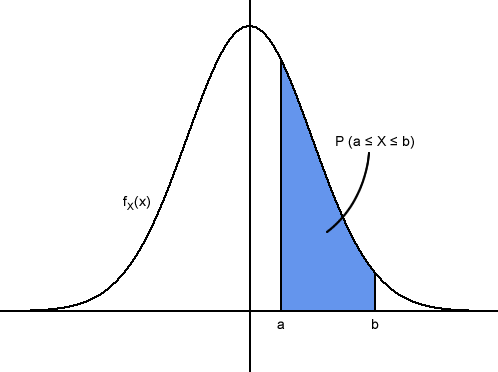
\includegraphics[scale=0.3]{Integral-dichte.png}
\end{center}
Die Gesammtfläche unter der Dichtefunktion muss gleich 1 sein.
\begin{equation}
P(-\infty \leq X \leq \infty) = \int_{-\infty}^{\infty} f(x) dx=1
\end{equation}
\subsection{Verteilungsfunktion}
\begin{equation}
F(x) = P(X \leq x) = \int_{-\infty}^x f(t) dx
\end{equation}
\subsubsection{Eigenschaften}
\begin{align}
P(a \leq X \leq b) = F(b)-F(a) \\
\lim_{x \rightarrow - \infty} F(x) = 0 \\
\lim_{x \rightarrow \infty} F(x) = 1 \\
F'(X) f(x), \text{falls f stetig}
\end{align}

\subsection{Erwartungswert, Varianz, Standardabweichung}
Erwartungswert von $X$:
\begin{equation}
E(x)=\int_{-\infty}^\infty x * f(x) dx
\end{equation}
Varianz von $X$:
\begin{equation}
V(x)=\int_{-\infty}^\infty (x - E(X))^2 * f(x) dx = E(X^2) - E(X)^2
\end{equation}
Standardabweichung von $X$:
\begin{equation}
\sigma(X) = \sqrt{V(X)}
\end{equation}
\subsection{Gleichverteilung}
\begin{definition}[stetige Gleichverteilung]
Die stetige Gleichverteilung auf dem Intervall$[s,t]$ ist gegeben durch die konstante Dichte $f(x)=\frac{1}{t-s}$ für $s \leq x \leq t$. 
\end{definition}
Schreibweise: $X \sim U[s,t]$ \\
$E(x) = \frac{s + t}{2}$ \\
$V(x) = \frac{1}{12}*(t-s)^2$

\subsection{Normalverteilung}
\subsubsection{Standardnormalverteilung}
\begin{definition}[Standardnormalverteilung]
Die Standardnormalverteilung ist gegeben durch die Dichte $\varphi(x) = \frac{1}{\sqrt{2\pi}}*e^{-\frac{x^2}{2}}$. Man nennt dies auch \textbf{Gauss'sche Glockenkurve}.
\end{definition}
Schreibweise: $X \sim N(0,1)$ \\
$E(x) = 0$ \\
$V(x) = 1$
\begin{center}
	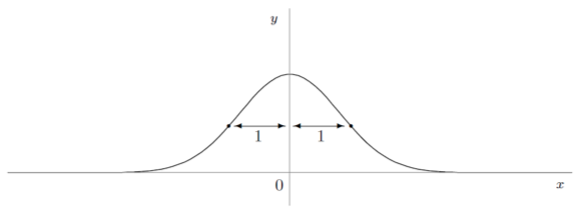
\includegraphics[scale=0.4]{standardnormalverteilung.png}
\end{center}
Die Verteilungsfunktion wird mit $\Phi$ bezeichnet: $\Phi(x) = \int_{-\infty}^x \varphi(t) dt$.
\subsubsection{Normalvertielung}
\begin{definition}[Normalverteilung]
Die Normalverteilung mit Parametern $\mu$ und $\sigma$ ist gegeben durch die Dichte $\varphi(x) = \frac{1}{\sqrt{2\pi\sigma^2}}*e^{-\frac{(x-\mu)^2}{2\sigma^2}}$.
\end{definition}
Schreibweise: $X \sim N(\mu,\sigma)$ \\
$E(x) = \mu$ \\
$V(x) = \sigma^2$
Die allgemeine Normalverteilung entsteht, in dem die Gauss'sche Glockenkurve horizontal um die Strecke $\mu$ verschoben wird und um den Faktor $\sigma>0$  horizental gestreckt wird: $\sigma_{\mu,\sigma}(x)=\frac{1}{\sigma}\varphi(\frac{x - \mu}{\sigma})$
\begin{center}
	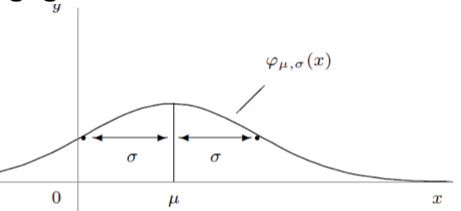
\includegraphics[scale=0.4]{normalvertielung.png}
\end{center}
Die Verteilungsfunktion wird mit $\Phi$ bezeichnet: $\Phi(x)_{\mu,\sigma} = \Phi(\frac{x-\mu}{\sigma})$.
\subsubsection{Matlab}
\begin{tabular}{l l}
	Dichte & normpdf($x$, $\mu$, $\sigma$) \\
	Verteilungsfunktion & normcdf($x$, $\mu$, $\sigma$) \\
\end{tabular}

\subsection{Quantil}
\begin{definition}[Quantil]
Gegeben sei ein $\alpha\in (0,1)$. Für welchen Wert $z_\alpha$ gilt $P(X \leq z_\alpha)=\alpha$? \\
So ein $z_\alpha$ heisst $\alpha$-Quantil (oder Perzentil)
\end{definition}
\begin{center}
	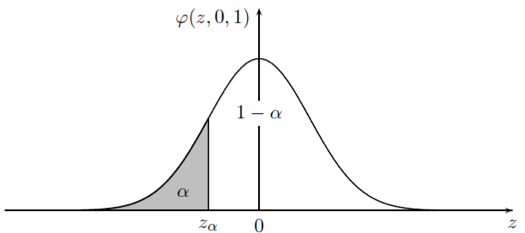
\includegraphics[scale=0.4]{quantil.png}
\end{center}
\subsubsection{Sigma-Regel}
Für $x \sim N(\mu,\sigma)$ gilt: \\
$P(\mid X - \mu \mid \leq \sigma) \approx 68.3\%$ : 1. Sigma-Regel \\
$P(\mid X - \mu \mid \leq 2\sigma) \approx 95.5\%$ : 2. Sigma-Regel \\
$P(\mid X - \mu \mid \leq 3\sigma) \approx 99.7\%$ : 3. Sigma-Regel
\begin{center}
	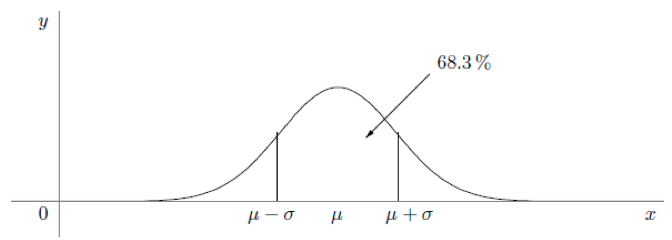
\includegraphics[scale=0.4]{sigma-regel.png}
\end{center}

\subsection{Exponentialverteilung}
Die Exponentialverteilung beschreibt zufällige Lebensdauernvon Geräten oder Wartezeiten auf zufällige Ereignisse.
\begin{definition}[Exponentialerteilung]
Die Wahrscheinlichkeit dass X einen Wert grösser als t annimt, sinkt exponentiell: $P(X \geq t) = e^{-\lambda t}$, $(t \geq 0)$ \\
Eine Zufallsvariable mit dieser Dichte heisst exponentiell verteilt mit Parameter $\lambda$.
\end{definition}
Schreibweise: $X \sim Exp(\lambda)$ \\
$E(x) = \frac{1}{\lambda}$ \\
$V(x) = \frac{1}{\lambda^2}$
\begin{center}
	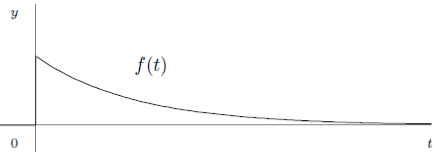
\includegraphics[scale=0.3]{exponentialverteilung.png}
\end{center}


\newpage
\section{Unabhängige Zufallsvariablen}
\subsection{Unabhängigkeit von Zufallsvariablen}
\begin{definition}[Unabhängige Zufallsvariablen]
Eine unendliche Folge von Zufallsvariablen heisst \textbf{(stochastisch) unabhängig}, wenn jede endliche Teilfolge davon stochastisch unabhängig ist. \\
Eine endliche Folge von Zufallsvariabeln $X_1$, \dots, $X_n$ heisst (stochastisch) unabhängig, wenn 
\begin{equation}
P(X_1 \leq x_1, X_2 \leq x_2, \dots, X_n \leq x_n) = P(X_1 \leq x_1) * P(X_2 \leq x_2), \dots, P(X_n \leq x_n)
\end{equation}
für alle $x_1, x_2, \dots, x_n \in \RN$
\end{definition}

\begin{satz} 
Es seien $X$ und $Y$ unabhängige diskrete Zufallsvariablen mit den Werten $\chi$ und $\Upsilon$ und Zähldichten $f_X$ und $f_Y$. \\
Weiter sei $g: \chi \times \Upsilon \rightarrow\ZN$. Dan gilt für alle $z \in \ZN$:
\begin{equation}
P(g(X,Y) = z) = \sum_{x \in \chi} \sum_{y\in \Upsilon:g(x,y)=z} f_X(x) * f_Y(y)
\end{equation}
\end{satz}

\begin{satz} 
Es seien $X$ und $Y$ unabhängige diskrete Zufallsvariablen mit den Werten $\chi$ und $\Upsilon$ und Zähldichten $f_X$ und $f_Y$. Dann hat die Summe $X + Y$ die Zähldichte
\begin{equation}
f_{X+Y}(z) = \sum_{x in \chi} f_X(x) * f_Y(z-x)
\end{equation}
Hierbei ist für $f_Y(y)=0$ für $y \notin \Upsilon$
\end{satz}
Die Zähldichte von $f_{X+Y}$ nennt man auch Faltung von $f_X$ und $f_Y$.

\begin{satz} 
Es seien $X$ und $Y$ unabhängige Zufallsvariablen sind, dan gilt
\begin{align}
X \sim Poi(\lambda_1), Y \sim Poi(\lambda_2) &\Rightarrow X + Y \sim Poi(\lambda_1 + \lambda_2) \\
X \sim Bin(n_1,p), Y \sim Bin(n_2,p) &\Rightarrow X + Y \sim Bin(n_1 + n_2, p)
\end{align}
\end{satz}

\begin{satz}[Additionstheorem der Normalverteilung]
Seien $X_1, X_2, \dots, X_n$ unabhängige, normal verteilte Zufallsvariablen eines Zufallsexperiments mit den Erwartungswerten $\mu_i$ und der Standardabweichung $\sigma_1$. Weiter seien$a_1,a_2, \dots, a_n$ belibige reelle Zahlen, nicht alle gleich 0. \\
Dann ist die Zufallsvariable $Y = a_1X_1 + a_2X_2 + \dots + a_nX_n$ auch normal verteilt mit Erwartungswert $a_1\mu_1,a_2\mu_2, \dots, a_n\mu_n$ und Varianz $a_1^2\sigma_1^2,a_2^2\sigma_2^2, \dots, a_n^2\mu_n^2$
\end{satz}

\subsection{Eigenschaft von Erwartungswert und Varianz}
Es seien $X$ und $Y$  Zufallsvariablen und $a, c \in \RN$.
Dan gilt:
\begin{align}
E(X + Y) = E(X) + E(Y) \\
E(aX) = aE(X) \\
E(X + c) = E(X) + c\\
V(X + c) = V(X)\\
V(aX) = a^2V(X)\\
\text{Falls X und Y unabhängig sind: } V(X + Y) = V(X) + V(Y) \\
\text{Wenn X diskret ist und } f_X \text{die Zählichte von X: } E(g(X)) = \sum_x g(x) * f_X(x) \\
\text{Wenn X stetig ist und } f_X \text{ ide Dichte von X: } E(g(X)) = \int_{-\infty}^\infty g(x) * f_X(x) dx
\end{align}

\subsection{die Ungleichung von Tschabyscheff}
\begin{satz}
Es sei X eine Zufallsvariable mit Erwartungswert $\mu$ und Varianz $\sigma^2$. Dann gilt für alle $k > 0$:
\begin{equation}
P(\mid X - \mu \mid \geq k) \leq \frac{\sigma^2}{k^2}
\end{equation}
\end{satz}
Diese Abschätzung gilt für alle möglichen Verteilungen von X. Sie ist deshalb in manchen Fällen recht grob.

\subsection{Grentzwertsätze}
\subsubsection{Gesetz der Grossen Zahlen}
Es sei E ein Ereignis eines Zufallexperiments, und sei $p$ die Wahrscheinlichkeit von E. Weiter bezeichne $X$ die Anzahl des Eintreffens von E bei $n$ unabhängigen Ausführungen dieses Experiments. Für jede beliebig kleine reelle Zahl $\epsilon > 0$ gilt dann:
\begin{equation}
P(\mid \frac{X}{n} - p \mid \geq \epsilon) \rightarrow 0 (n \rightarrow \infty)
\end{equation}
\subsubsection{Zentraler Grenzwertsatz}
Es sei $X_1, X_2,$ \dots eine Folge von unabhängigen Zufallsvariablen eines  Wahrscheinlichkeitsraumes, welche alle dieselbe Verteilung mit Erwartungswert $\mu$ und Varianz $\sigma^2$ haben. Dan gilt für grosse $n$: \\
Die Summe $S_n = X_1 + \dots + X_n$ besitzt näherungsweise die Normalverteilung $N(\mu_n, \sigma_n)$ mit $\mu_n = n * \mu$ und $\sigma_n = \sqrt{n} * \sigma$. Es gilt also näherungsweise $ \frac{S_n - \mu_n}{\sqrt{n} * \mu} \sim N(0,1)$. \\
Präzise gilt für alle $z \in \RN$:
\begin{equation}
P(\frac{S_n - n\mu}{\sqrt{n}\sigma} \leq z) \rightarrow \Phi(z) (n \rightarrow \infty)
\end{equation}
\subsubsection{Grenzwertsatz von de Moivre und Laplace}
Für grosse $n$ ist
\begin{equation}
P(a \leq X \leq b) \approx \Phi (\frac{b - np}{\sqrt{np(1-p)}}) - \Phi (\frac{a - np}{\sqrt{np(1-p)}})
\end{equation}
Diese Approximation ist für $n > \frac{9}{p(1-p)}$ hinfreichend genau. \\
Etwas genauer wird es mit der sogenannten \textbf{Stetigkeitskorrektur}:
\begin{equation}
P(a \leq X \leq b) \approx \Phi(\frac{b + \frac{1}{2} - np}{\sqrt{np(1-p)}}) - \Phi(\frac{a - \frac{1}{2} - np}{\sqrt{np(1-p)}})
\end{equation}

\newpage
\section{Aspekte der induktiven Statistik}

% Inhalt Ende 
\end{document} 